\documentclass[lightblue, notheorems, xcolor=dvipsnames]{beamer}
%\usepackage{beamerthemeshadow}
\usetheme{Madrid}

\usepackage[english]{babel}
\usepackage[utf8]{inputenc}
\usepackage[T1]{fontenc}
\usepackage{amsmath, amssymb, amsthm, amsfonts} %einige hilfreiche Mathe-Pakete
\setbeamertemplate{theorems}[ams style]
\usepackage{tabularx, multirow} %fuer Tabellen
\usepackage{graphicx, tikz} %Grafiken
\usepackage{setspace} %Paket f\"ur das Formatieren von Quellen unten auf einer Folie
\newcommand{\diff}{\mathop{}\!\mathrm{d}}
\usepackage[T1]{fontenc}

% Algorithm
\usepackage[ruled,vlined]{algorithm2e}
\usepackage{algpseudocode}
\usepackage{algorithmicx}



% BIlder
\setbeamertemplate{caption}[numbered]
\usepackage{subcaption}
%\usepackage{subfig}
\usepackage{graphicx}
\usepackage{float}

\usepackage{comment}

% Ausblenden Navigation
\beamertemplatenavigationsymbolsempty

% definiere Enviroments
\theoremstyle{definition}
\newtheorem{defi}{Definition}[section]
\newtheorem{idea}{Idee}[section]
\theoremstyle{plain}
\newtheorem{theo}[defi]{Satz}
\newtheorem{coroll}[defi]{Korollar}%
\newtheorem{lem}[defi]{Lemma}%
\newtheorem{aim}[defi]{Ziel}
%\newtheorem*{proof}{Beweis}%[theorem]

\theoremstyle{example}
\newtheorem{remark}[defi]{Bemerkung}%
\newtheorem{examp}[defi]{Beispiel}%
\newtheorem*{lsg}{Lösung}


\DeclareMathOperator*{\argmax}{argmax}


\iffalse
\expandafter\def\expandafter\insertshorttitle\expandafter{%
    \insertshorttitle\hfill%
    \insertframenumber\,/\,\inserttotalframenumber}
\fi



\SetKwRepeat{Do}{do}{while}%
\begin{document}
   %\maketitle  %erstellt Titelseite mit oben stehenden Informationen
  % optional: mit 
  \author{Bella My Phuong Quynh Duong}
  \date{September 26, 2023} %Datum des Vortrags eintragen
  \institute{Heinrich-Heine University D\"usseldorf}
  \title[Structure-Preserving Multi-Scale Methods
  for Complex Fluids]{Numerical Solution with Spectral Method for Smoluchowski Equation on $S^2$}
  
  \begin{frame}
  	\titlepage
  	\begin{figure}[htpb]
  		\begin{center}
  			
\includegraphics[width=0.2\textwidth]{logo.png}
  		\end{center}
  	\end{figure}
  \end{frame}
\begin{frame}
   \frametitle{Table of Contents}
\tableofcontents %dieser Befehl erzeugt das Inhaltsverzeichnis
\end{frame}

\AtBeginSection[]
{
	\begin{frame}<beamer>
		\frametitle{Overview}
		\tableofcontents[currentsection]
	\end{frame}
}

\section{Motivation}
\begin{frame}
    Guazzelli et al examined a dilute suspension of rod-like particles influenced by gravity.
\begin{columns}
	\begin{column}{0.5\textwidth}
		\begin{itemize}
			\item In an initially homogeneous suspension, rod-like particles form clusters where they are denser.
			\item The clusters create downward flows balanced by upward flows.
			\item Particles in a cluster mostly align with gravity, occasionally flipping.
		\end{itemize}
	\end{column}
	\begin{column}{0.5\textwidth}
		\begin{figure}[H]
			\centering
			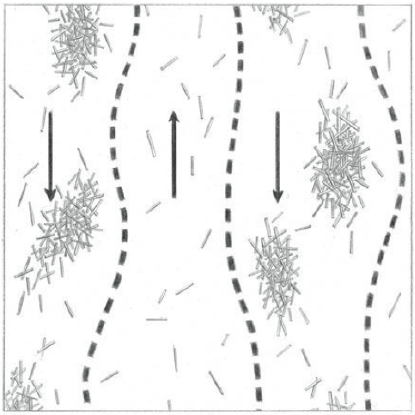
\includegraphics[scale=0.5]{Bilder/Bild_Particles}
		\end{figure}
	\end{column}
\end{columns}
\end{frame}

\begin{frame}{Mathematical Model for the Sedimentation of Rod-Like Particles}
	\scriptsize
\text{Coupling of a kinetic Smoluchowski equation with Navier-Stokes equation}
\begin{align*}
	\textcolor{blue}{\partial_t f}+ \textcolor{red}{\nabla_{\boldsymbol{x}} \cdot(\boldsymbol{u} f)} & +\textcolor{blue}{\nabla_{\boldsymbol{n}} \cdot\left(P_{\boldsymbol{n}^{\perp}} \nabla_{\boldsymbol{x}} \boldsymbol{u} \boldsymbol{n} f\right)}- \textcolor{red}{\nabla_{\boldsymbol{x}} \cdot\left((I+\boldsymbol{n} \otimes \boldsymbol{n}) e_3 f\right)} \\
	& =\textcolor{blue}{D_r \Delta_n f}+\gamma \nabla_{\boldsymbol{x}} \notag \cdot(I+\boldsymbol{n} \otimes \boldsymbol{n}) \nabla_{\boldsymbol{x}} f, \\
	\sigma & =\int_{S^{d-1}}(\text{d} \; \boldsymbol{n} \otimes \boldsymbol{n}-I) f d \boldsymbol{n},  \\
	\operatorname{Re}\left(\partial_t \boldsymbol{u}+\left(\boldsymbol{u} \cdot \nabla_{\boldsymbol{x}}\right) \boldsymbol{u}\right) & =\Delta_{\boldsymbol{x}} \boldsymbol{u}-\nabla_{\boldsymbol{x}} p+\delta \gamma \nabla_{\boldsymbol{x}} \cdot \sigma-\delta \int_{S^{d-1}} f d \boldsymbol{n} \, e_3, \\
	\nabla_{\boldsymbol{x}} \cdot \boldsymbol{u} & =0,
\end{align*}
where $f = f(\boldsymbol{x}, t, \boldsymbol{n}), \boldsymbol{x} \in \mathbb{R}^3 , \boldsymbol{n} \in  S^2$ is a density distribution function of particle orientation. $D_r, \gamma, \delta$ and $Re$ are non-dimensional parameters.
\begin{beamercolorbox}[sep=1em,wd=\linewidth,right]{}
	\tiny{Helzel $\&$ Tzavaras, 2017}
\end{beamercolorbox}
Here we consider the case $\gamma = 0$.
\end{frame}


\begin{frame}{Status of Project}
	\scriptsize
    \begin{block}{So far...}
    	\begin{itemize}
    		\item  Investigate hierarchy of moment equations for simplified model with \textcolor{cyan}{$f$ on $S^1$}
    		\begin{itemize}
    		\item <1->  Transform high dimensional scalar PDE (in space and orientation) into a lower dimensional system of moment equations (in
    		space)
    	   \item <2-> Investigate accuracy of moment closure system
    	    \end{itemize}
    	\end{itemize}
       	   Dahm, Helzel, MMS 2022, Dahm, Giesselmann, Helzel, JCP 2024
    \end{block}
	\begin{block}{Now}
		\begin{itemize}
			\item <3-> Derive and approximate hierarchies of moment equations for the coupled kinetic-fluid model with \textcolor{cyan}{$f$ on $S^2$}.
		\end{itemize}
	\end{block}
\end{frame}
%%%%%%%%%%%%%%%%%%%%%%%%%%%%%%%%%%%%%%%%%%%%%%%%%%%%%%
\begin{comment}
\begin{frame}{Spectral method}
	\scriptsize
	Consider the drift-diffusion equation
	\begin{align}
		\textcolor{blue}{\partial_t f}+ \textcolor{gray!80}{\nabla_{\boldsymbol{x}} \cdot(\boldsymbol{u} f)} & +\textcolor{blue}{\nabla_{\boldsymbol{n}} \cdot\left(P_{\boldsymbol{n}^{\perp}} \nabla_{\boldsymbol{x}} \boldsymbol{u} \boldsymbol{n} f\right)}-\textcolor{gray!80}{\nabla_{\boldsymbol{x}} \cdot\left((I+\boldsymbol{n} \otimes \boldsymbol{n}) e_3 f\right)} \notag \\
		& = \textcolor{blue}{D_r \Delta_n f}+\textcolor{gray!80}{\gamma \nabla_{\boldsymbol{x}} \cdot(I+\boldsymbol{n} \otimes \boldsymbol{n}) \nabla_{\boldsymbol{x}} f} \label{SmochEq_kurz}
	\end{align}
	with externally imposed velocity gradient $\nabla_x. \boldsymbol{u}_{\mathrm{ext}}$\\
	\vspace{12pt}
	\pause
	In spherical coordinates
	\begin{align}
		\underbrace{\sin \theta \partial_t f}_{[1]} + \underbrace{\partial_\phi\left(a(\phi, \theta) f\right)+\partial_\theta\left(b(\phi, \theta) f\right)}_{[2]} = \underbrace{D_r \left(\partial_\phi\left(\frac{1}{\sin \theta} \partial_\phi f\right)+\partial_\theta\left(\sin \theta \partial_\theta f\right)\right)}_{[3]}, \label{Smoch_S2}
	\end{align}	
	with $\phi \in [0, 2 \pi]$ and $\theta \in [0, \pi]$.\\
	\vspace{12pt}
	\pause
  Ansatz for our \textcolor{cyan}{spectral method}
\begin{align}
	f(x,t,\phi, \theta) \approx f_0(x,t) \cdot P_0^0 + \sum_{n=1}^{N} \sum_{k=-2n}^{2n} c^k_{2n}(x,t) \cdot P^k_{2n}(\phi, \theta), \label{ansatz}
\end{align}
where $P^k_{2n}(\phi, \theta)$ are harmonic polynomial basis functions.  %, i.e. are eigenfunctions of Laplace Beltrami operator.
\end{frame}

\begin{frame}{Example}
	\scriptsize
	For $N=1$ we obtain
	\begin{equation}
		\left(\begin{array}{c}
			f_0(t) \\
			c_2^{-2}(t) \\
			c_2^{-1}(t) \\
			c_2^0(t) \\
			c_2^1(t) \\
			c_2^2(t)
		\end{array}\right)^{\prime} - A \cdot
		\left(\begin{array}{c}
			f_0(t) \\
			c_2^{-2}(t) \\
			c_2^{-1}(t) \\
			c_2^0(t) \\
			c_2^1(t) \\
			c_2^2(t)
		\end{array}\right) = -6 D_r \cdot
		\left(\begin{array}{c}
			0 \\
			c^{-2}_2(t) \\
			c_2^{-1}(t) \\
			c_2^0(t) \\
			c_2^1(t) \\
			c_2^2(t)
		\end{array}\right),
	\end{equation}
\end{frame}

\begin{frame}
	where the matrix $A$ has the form \\
	\vspace{8pt}
	\begin{multline*}
		\resizebox{\textwidth}{!}{%
			\(
			\begin{pmatrix}
				\vspace{12pt}
				0 & 0 & 0 & 0 & 0 & 0 \\
				\vspace{12pt}
				\frac{1}{5}\sqrt{15}(u_x-v_y) & \frac{1}{7}(u_x+v_y-2w_z) & \frac{1}{7}(-5u_z+2w_x) & \frac{1}{7}\sqrt{3}(-u_x+v_y) & \frac{1}{7}(5v_z-2w_y) &  (u_y -v_x) \\
				\vspace{12pt}
				\frac{1}{5}\sqrt{15}(-u_z-w_x) & \frac{1}{7}(2u_z-5w_x) & \frac{1}{7}(u_x-2v_y+w_z) & \frac{1}{7}\sqrt{3}(-4u_z+3w_x) & \frac{1}{7}(5u_y-2v_x) &  \frac{1}{7} \left(2v_z-5w_y\right) \\
				\vspace{12pt}
				\frac{1}{5}\sqrt{5}(-u_x-v_y+2w_z) & \frac{1}{7}\sqrt{3}(-u_x+v_y) & \frac{1}{7}\sqrt{3}(3u_z-4w_x) & \frac{1}{7}(-u_x-v_y+2w_z) & \frac{1}{7}\sqrt{3}(-3v_z-4w_y) & \frac{1}{7} \sqrt{3}\left(-u_y-v_x\right) \\
				\vspace{12pt}
				\frac{1}{5}\sqrt{15}(-v_z-w_y) & \frac{1}{7}(-2v_z+5w_y) & \frac{1}{7}(-2u_y+5v_x) & \frac{1}{7}\sqrt{3}(-4v_z+3w_y) & \frac{1}{7}(-2u_x+v_y+w_z) &  \frac{1}{7} \left(2u_z-5w_x\right)\\
				\vspace{12pt}
				\frac{1}{5}\sqrt{15}(u_y+v_x) & (-u_y+v_x) & \frac{1}{7}(-5v_z+2w_y) & \frac{1}{7}\sqrt{3}(-u_y-v_x) & \frac{1}{7}(-5u_z+2w_x) & \frac{1}{7} \left(u_x+v_y-2w_z\right)
			\end{pmatrix}
			\).
		}
	\end{multline*}
\end{frame}
\end{comment}



%\section{Theoretical background}
\begin{frame}\frametitle{Spherical Harmonics}
	\small
		\begin{theorem}
			Let $P^{i_1}_{n_1}(\phi, \theta)$ and $P^{i_2}_{n_2}(\phi, \theta)$ are two different harmonic polynomial basis functions. Then the integral over the sphere is equal to zero
			\begin{align*}
				\int_{0}^{2\pi} \int_{0}^{\pi} P^{i_1}_{n_1} \cdot P^{i_2}_{n_2} \cdot \sin(\theta) d\theta d\phi = 0.
			\end{align*}
		\end{theorem}

		\begin{theorem}
			Let $P^i_{2n}$ with $n = 0, ..., \infty$ and $i = n, ..., -n$ be the normalized harmonic polynomial basis functions. The integral over $S^2$ of the normalized basis functions is equal to one.
		\end{theorem}

	The properties show that the spherical harmonics on the unit sphere form an orthonormal basis, which means that they are orthogonal to each other, and the integral over the unit sphere of each individual spherical harmonic is equal to 1 when they are normalized.
\end{frame}

\begin{frame}
	\begin{definition}
		The \textbf{Laplace-Beltrami operator} on the unit sphere $S^2$ is given by
		\begin{align*}
			\Delta_{S^2} f = \frac{1}{\sin ^2 \theta} \partial_{\phi \phi} f + \frac{1}{\sin \theta} \partial_\theta\left(\sin \theta \partial_\theta f\right).
		\end{align*}
		The spherical harmonic function are the eigenfunctions of Laplace-Beltrami operator with the eigenvalues $(- \ell (\ell +1),\ell \in \mathbb{N}_0)$(see \cite{zbMATH01218597})
		\begin{align*}
			\Delta_{S^2}P^i_n = -\ell(\ell+1) P^i_n,
		\end{align*}
		with $n = 0, ..., \infty$ and $i = n ,..., -n$.
	\end{definition}
\end{frame}

%\begin{columns}[T, totalwidth=\textwidth]
%	\begin{column}{0.44\textwidth}
%		\begin{definition}
%			\begin{itemize}
%				\item x: Input image
%				\item z: Internal latent vector
%				\item $\phi$:  Encoder model parameter
%				\item $\theta$:  Decoder model parameter
%			\end{itemize}
%		\end{definition}
%	\end{column}
%	\begin{column}{0.53\textwidth}
%		\begin{definition}
%			\begin{itemize}
%				\item $q_{\phi}(z|x)$: Probability distr. (Encoder)
%				\item $p_{\theta}(x|z)$: Probability distr. (Decoder)
%				\item $KL(P,Q) = \sum_{x \in X}^{} P(x) log(\frac{P(x)}{Q(x)})$	
%			\end{itemize}
%		\end{definition}
%	\end{column}
%\end{columns}
\section{Spectral method}
\begin{frame}
	\scriptsize
	Consider the drift diffusion term
	\begin{align}
		\textcolor{blue}{\partial_t f}+ \textcolor{gray!80}{\nabla_{\boldsymbol{x}} \cdot(\boldsymbol{u} f)} & +\textcolor{blue}{\nabla_{\boldsymbol{n}} \cdot\left(P_{\boldsymbol{n}^{\perp}} \nabla_{\boldsymbol{x}} \boldsymbol{u} \boldsymbol{n} f\right)}-\textcolor{gray!80}{\nabla_{\boldsymbol{x}} \cdot\left((I+\boldsymbol{n} \otimes \boldsymbol{n}) e_3 f\right)} \notag \\
		& = \textcolor{blue}{D_r \Delta_n f}+\textcolor{gray!80}{\gamma \nabla_{\boldsymbol{x}} \cdot(I+\boldsymbol{n} \otimes \boldsymbol{n}) \nabla_{\boldsymbol{x}} f} \label{SmochEq_kurz}
	\end{align}
    with externally imposed velocity gradient $\nabla_x \boldsymbol{u}_{\mathrm{ext}}$\\
	\vspace{12pt}
	\pause
	In spherical coordinates
	\begin{align}
		\sin \theta \partial_t f + \partial_\phi\left(a(\phi, \theta) f\right)+\partial_\theta\left(b(\phi, \theta) f\right) = D_r \left(\partial_\phi\left(\frac{1}{\sin \theta} \partial_\phi f\right)+\partial_\theta\left(\sin \theta \partial_\theta f\right)\right), \label{Smochluch_S2}
	\end{align}
	with $\phi \in [0, 2 \pi]$ and $\theta \in [0, \pi]$\\
	\vspace{12pt}
	\pause
   	Ansatz for our \textcolor{cyan}{spectral method}
	\begin{align}
		f(\phi, \theta, t) \approx f_0(t) \cdot P_0^0 + \sum_{n=1}^{N} \sum_{i=-2n}^{2n} c^i_{2n}(t) \cdot P^i_{2n}(\phi, \theta), \label{ansatz}
	\end{align}
	where $P^i_{2n}(\phi, \theta)$ are harmonic polynomial basis functions %, i.e. are eigenfunctions of Laplace Beltrami operator.
\end{frame}

%%%%%%%%%%%%%%%%%%%%%%%%%
% Von Frau Helzel's Idee
%%%%%%%%%%%%%%%%%%%%%%%%%

\begin{frame}
	Scalar product on $S^2$
	\begin{align*}
		(g,h)_{S^2} := \int_{0}^{2\pi} \int_{0}^{\pi} g(\phi, \theta) h(\phi, \theta) \cdot \sin(\theta) d\theta d\phi
	\end{align*}

	\begin{figure}
		\small
		\begin{minipage}{0.46\textwidth}
			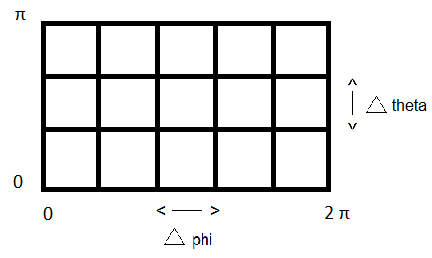
\includegraphics[scale=0.5]{Bilder/Gitter_phi_theta}
		\end{minipage}
		\hfill 
		\begin{minipage}{0.5\textwidth}
			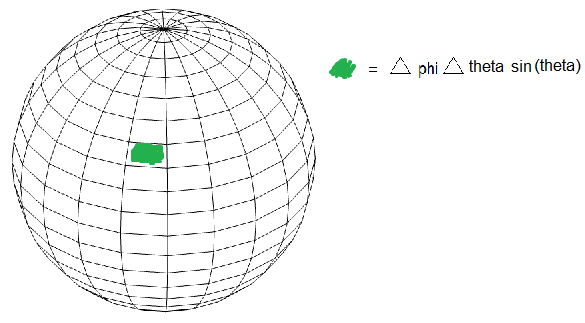
\includegraphics[scale=0.48]{Bilder/Kugel_mit_grid}
		\end{minipage}
	\caption{Grid on sphere}
	\end{figure}
\end{frame}



%%%%%%%%%%%%%%%%%%%%%%
% Properties
%%%%%%%%%%%%%%%%%%%%%%

\begin{frame}{Properties of harmonic polynomial basis functions}
	\begin{itemize}
		\item $\Delta_{S^2}P^i_n = -n(n+1) P^i_n$
		\vspace{12pt}
		\item $	f(\phi, \theta) = f_0 \cdot P_0^0 + \sum_{n=1}^{\infty} \sum_{i=-2n}^{2n} c^i_{2n} \cdot P^i_{2n}(\phi, \theta)$
		\vspace{12pt}
		\item $(P^i_n, P^l_m)_{S^2} = 0, \forall i \neq l \; \text{or} \; n \neq m$
		\vspace{12pt}
		\item $	(P^i_n, P^i_n)_{S^2} = 1$
	\end{itemize}
\end{frame}

\begin{frame}{Harmonic polynomial basis functions}
	\scriptsize
	Basis function ${P}^{i}_{n}(\phi, \theta)$, $n = 0, ..., \infty$ and $i = n, ..., -n$ are computed from orthogonal polynomials (Legendre polynomials). 
	\vspace{20pt}
	\begin{figure}
		\centering
		\subfloat[$P^0_0$]{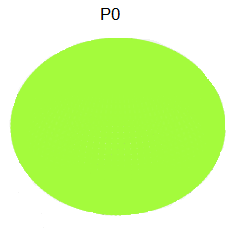
\includegraphics[width=2cm,height=2cm]{Bilder/P0_Kugel}}
		\qquad
		\subfloat[$P^{-1}_2$]{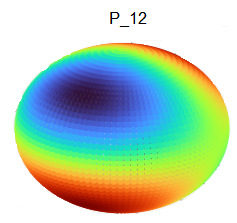
\includegraphics[width=2cm,height=2cm]{Bilder/P_12_Kugel}}
		\qquad
		\subfloat[$P^0_2$]{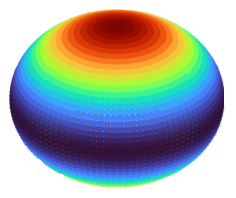
\includegraphics[width=2cm,height=2cm]{Bilder/P02_Kugel}}
		\qquad
		\subfloat[$P^{-1}_4$]{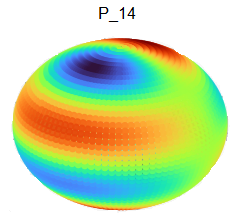
\includegraphics[width=2cm,height=2cm]{Bilder/P_14_Kugel}}
		\caption{Some harmonic polynomial basis functions}
	\end{figure}

	\begin{minipage}[b]{0.4\textwidth}
		\begin{table}[H]
			\tiny
			\begin{tabular}{|c|c|}
				\hline
				0th order & 2nd order \\
				\hline
				& $P^{-2}_2 = \sqrt{\frac{15}{16\pi}}\sin^2(\theta)\cos(2\phi)$ \\
				& $P^{-1}_2 = \sqrt{\frac{15}{4\pi}}\sin(\theta)\cos(\theta)\cos(\phi)$ \\
				$P^0_0 = \sqrt{\frac{1}{4\pi}} \cdot 1$ & $P^0_2 = \sqrt{\frac{45}{16\pi}}\cos^2(\theta) - \frac{1}{3}$ \\
				& $P^1_2 = \sqrt{\frac{15}{4\pi}}\sin(\theta)\cos(\theta)\sin(\phi)$\\
				& $P^2_2 = \sqrt{\frac{15}{16\pi}}\sin^2(\theta)\sin(2\phi)$\\
				\hline
			\end{tabular}
		\end{table}
	\end{minipage}
\end{frame}


\begin{comment}
\begin{frame}{Harmonic polynomial basis functions}
	\scriptsize
	Let ${P}^{i}_{n}(\phi, \theta)$ with $n = 0, ..., \infty$ and $i = n, ..., -n$ be the basis function
	\begin{align*}
		TODO
	\end{align*}
	The scalar product of any two basis functions over sphere is defined as follows
	\begin{align*}
		<P^i_n, P^l_m>_{S^2} = \int_{0}^{2\pi} \int_{0}^{\pi} P^{i}_{n}(\phi, \theta) \cdot P^{l}_{m}(\phi, \theta) \cdot \sin(\theta) d\theta d\phi.
	\end{align*}
\end{frame}
\end{comment}

\begin{comment}
\begin{frame}{Properties of harmonic polynomial basis functions}
	\scriptsize
	\begin{block}{Property 1}
		Let $P^{i}_{n}(\phi, \theta)$ and $P^{l}_{m}(\phi, \theta)$ are two different harmonic polynomial basis functions. Then
		\begin{align*}
			<P^i_n, P^l_m>_{S^2} = 0,
		\end{align*}
	for $i \neq l$ or $n \neq m$.
	\end{block}
	
	\begin{block}{Property 2}
		Let $P^i_{n}$ be the normalized harmonic polynomial basis functions. Then
		\begin{align*}
			<P^i_n, P^i_n>_{S^2} = 1.
		\end{align*}
	\end{block}

	\begin{block}{Property 3}
		The spherical harmonic function are the eigenfunctions of Laplace-Beltrami operator with the eigenvalues $(- n (n +1),n \in \mathbb{N}_0)$(see \cite{zbMATH01218597})
		\begin{align*}
			\Delta_{S^2}P^i_n = -n(n+1) P^i_n.
		\end{align*}
	\end{block}
\end{frame}
\end{comment}

%%%%%%%%%%%%%%%%%%%%%%%%%%%%%%%%%%%%%%
% Back to the spectral method
%%%%%%%%%%%%%%%%%%%%%%%%%%%%%%%%%%%%%%

\begin{frame}{Spectral method}
	\scriptsize
	Kinetic Smochluchowski equation:
	\begin{align}
		\underbrace{\sin \theta \partial_t f}_{[1]} + \underbrace{\partial_\phi\left(a(\phi, \theta) f\right)+\partial_\theta\left(b(\phi, \theta) f\right)}_{[2]} = \underbrace{D_r \left(\partial_\phi\left(\frac{1}{\sin \theta} \partial_\phi f\right)+\partial_\theta\left(\sin \theta \partial_\theta f\right)\right)}_{[3]} \label{Smoch_S2}
	\end{align}	
	Ansatz: $f(\phi, \theta, t) = f_0(t) \cdot P_0^0 + \sum_{n=1}^{N} \sum_{i=-2n}^{2n} c^i_{2n}(t) \cdot P^i_{2n}(\phi, \theta)$
 	\vspace{12pt}
 	\begin{itemize}
 		\item Insert ansatz for $f$ in (\ref{Smoch_S2}) 
 		\item Multiply consecutively with all basis functions used in the ansatz and integrate the resulting equations over $\phi$ and $\theta$
 	\end{itemize}
\end{frame}

\begin{frame}{Example for a General Model}
	\scriptsize
	For  $f(\phi, \theta, t) = c^0_0(t) + \sum_{i=-2}^{2} c^i_{2}(t) \cdot P^i_{2}(\phi, \theta)$ we obtain
		\begin{equation}
		\left(\begin{array}{c}
			f_0(t) \\
			c_2^{-2}(t) \\
			c_2^{-1}(t) \\
			c_2^0(t) \\
			c_2^1(t) \\
			c_2^2(t)
		\end{array}\right)^{\prime} - A \cdot
		\left(\begin{array}{c}
			f_0(t) \\
			c_2^{-2}(t) \\
			c_2^{-1}(t) \\
			c_2^0(t) \\
			c_2^1(t) \\
			c_2^2(t)
		\end{array}\right) = -6 D_r \cdot
		\left(\begin{array}{c}
			0 \\
			c^{-2}_2(t) \\
			c_2^{-1}(t) \\
			c_2^0(t) \\
			c_2^1(t) \\
			c_2^2(t)
		\end{array}\right)
	\end{equation}
\end{frame}


%%%%%%%%%%%%%%


\begin{frame}
where the matrix $A$ has the form \\
\vspace{8pt}
\begin{multline*}
	\resizebox{\textwidth}{!}{%
		\(
		\begin{pmatrix}
			\vspace{12pt}
			0 & 0 & 0 & 0 & 0 & 0 \\
			\vspace{12pt}
			\frac{1}{5}\sqrt{15}(u_x-v_y) & \frac{1}{7}(u_x+v_y-2w_z) & \frac{1}{7}(-5u_z+2w_x) & \frac{1}{7}\sqrt{3}(-u_x+v_y) & \frac{1}{7}(5v_z-2w_y) &  (u_y -v_x) \\
			\vspace{12pt}
			\frac{1}{5}\sqrt{15}(-u_z-w_x) & \frac{1}{7}(2u_z-5w_x) & \frac{1}{7}(u_x-2v_y+w_z) & \frac{1}{7}\sqrt{3}(-4u_z+3w_x) & \frac{1}{7}(5u_y-2v_x) &  \frac{1}{7} \left(2v_z-5w_y\right) \\
			\vspace{12pt}
			\frac{1}{5}\sqrt{5}(-u_x-v_y+2w_z) & \frac{1}{7}\sqrt{3}(-u_x+v_y) & \frac{1}{7}\sqrt{3}(3u_z-4w_x) & \frac{1}{7}(-u_x-v_y+2w_z) & \frac{1}{7}\sqrt{3}(-3v_z-4w_y) & \frac{1}{7} \sqrt{3}\left(-u_y-v_x\right) \\
			\vspace{12pt}
			\frac{1}{5}\sqrt{15}(-v_z-w_y) & \frac{1}{7}(-2v_z+5w_y) & \frac{1}{7}(-2u_y+5v_x) & \frac{1}{7}\sqrt{3}(-4v_z+3w_y) & \frac{1}{7}(-2u_x+v_y+w_z) &  \frac{1}{7} \left(2u_z-5w_x\right)\\
			\vspace{12pt}
			\frac{1}{5}\sqrt{15}(u_y+v_x) & (-u_y+v_x) & \frac{1}{7}(-5v_z+2w_y) & \frac{1}{7}\sqrt{3}(-u_y-v_x) & \frac{1}{7}(-5u_z+2w_x) & \frac{1}{7} \left(u_x+v_y-2w_z\right)
		\end{pmatrix}
		\)
	}
\end{multline*}
\end{frame}





\begin{comment}
\begin{frame}
	\scriptsize
	
	The Laplace Beltrami operator (\cite{zbMATH07295185}) on the unit sphere $S^2$ is given by
	\begin{align}
		\Delta_{S^2} f = \frac{1}{\sin ^2 \theta} \partial_{\phi \phi} f + \frac{1}{\sin \theta} \partial_\theta\left(\sin \theta \partial_\theta f\right). \label{laplace_eq}
	\end{align}
	From property 3 and the equation $(\ref{laplace_eq})$, it follows for the term (3)
	\begin{align*}
		\Delta_{S^2} P^i_{2n} = -n(n+1)P^i_{2n}.
	\end{align*}
	For the term $(1)$ and $(2)$, we inserting (5) in (4), multiplying with each basis function and integrate it over $S^2$. We derive a system of ODEs for the coefficients
	\scriptsize
	\begin{equation}
		\left(\begin{array}{c}
			f_0 \\
			c_2^{-2} \\
			\vdots \\
			c_{2n}^i
		\end{array}\right)^{\prime}=A\left(\begin{array}{c}
			f_0 \\
			c_2^{-2} \\
			\vdots \\
			c_{2n}^i
		\end{array}\right),
	\end{equation}
with $A \in \mathbb{R}^{cnxcn}$
\begin{equation*}
	c n= \begin{cases}\text { order }=2: & cn= 2 \cdot \text {order}+2 \\ \text { order }=\text {even: } & c2=6 \\  &c n=c2 \\ &c n=c2+\sum_{i=4}^{order}(2 i+1)\end{cases}
\end{equation*}
\end{frame}

%%%%%%%%%%%%%%%%%%
% Example
%%%%%%%%%%%%%%%%%%

\begin{frame}
	\centering
	Example: Shear flow
\end{frame}

\begin{frame}{Example: Shear flow}
	\scriptsize
	Consider the Smoluchowski equation $(\ref{Smoch_S2})$ with the velocity gradient 
	\begin{align*}
		\vec{u}=\left(\begin{array}{l}
			u(x,y,z) \\
			v(x,y,z) \\
			w(x,y,z)
		\end{array}\right),
		\nabla_x \vec{u}_{\mathrm{ext}}=\left(\begin{array}{lll}
			u_{x} & u_{y} & u_{z} \\
			v_{x} & v_{y} & v_{z} \\
			w_{x} & w_{y} & w_{z}
		\end{array}\right)=\left(\begin{array}{ccc}
			0 & 1 & 0 \\
			0 & 0 & 0 \\
			0 & 0 & 0
		\end{array}\right) .
	\end{align*}
	With the given velocity gradient it follows
	\begin{align}
		\partial_{t}\left(\sin \theta f\right) &+ \partial_\theta\left(\sin \phi \cos \phi \sin ^2 \theta \cos \theta f\right)+ \partial_\phi\left(- \sin \theta \sin ^2 \phi f \right) \nonumber \\
		&=D_{r}\left(\partial_\theta \left(\sin \theta \partial_\theta f\right)+ \partial_\phi\left(\frac{1}{\sin \theta} \partial_\phi f\right)\right). \label{smoEq} 
	\end{align}
	Consider the ansatz with the zeroth order
	\begin{align}
		f(\phi, \theta, t)= f_0(t) \cdot P_0^0 \label{ansatz_0nd}.
	\end{align}

	Insert the ansatz (\ref{ansatz_0nd}) in (\ref{smoEq})
	\begin{align}
		\partial_{t}(f_0(t) \cdot P_0^0)+\frac{1}{\sin \theta}\left(\partial_\theta(\ldots)+\partial_\phi(\ldots)\right)=\frac{1}{\sin \theta} D_r \left(\ldots \right) \label{eq_mitAnsatz}.
	\end{align}
\end{frame}

\begin{frame}
	\scriptsize
	We know
	\begin{align*}
		\Delta_{S^2} P_0^0(\phi, \theta) = \frac{1}{\sin \theta} D_r (\ldots) = \lambda_{2n,i} \cdot P^{0}_0(\phi, \theta),
	\end{align*}
	where $\lambda_{2n,i}$ is the corresponding eigenvalue.\\
	Since $P_0^0(\phi, \theta) = 1$ does not depend on $\phi$ and $\theta$, the partial derivatives will be zero
	\begin{align}
		\Delta_{S^2} P_0^0(\phi, \theta) = 0.
	\end{align}
	Consider the rest of the equation (\ref{eq_mitAnsatz})
	\begin{align*}
		\underbrace{\partial_{t}(f_0(t) \cdot P_0^0)}_{(1)}+ \underbrace{\frac{1}{\sin\theta}\left( \partial_\theta(\sin \phi \cos \phi \sin ^2 \theta \cos \theta \cdot f_0(t) \cdot P_0^0)+ \partial_\phi(- \sin \theta \sin ^2 \phi \cdot f_0(t) \cdot P_0^0)\right)}_{(2)}.
	\end{align*}
	It is
	\begin{align*}
		\partial_t\left(f_0(t) \cdot P^0_0\right)=f_0^{\prime}(t).
	\end{align*}
	Let $z(\phi, \theta) := (2)$
\end{frame}

\begin{frame}
	\scriptsize
	Project the solution $z(\phi, \theta)$ onto all polynomials to find out which polynomial are needed
	\begin{align*}
		\int_{0}^{2\pi} \int_{0}^{\pi} z(\phi, \theta) \cdot P^{-2}_2(\phi, \theta) \, \sin \theta d\theta d\phi &\overset{Maple}{=} 0 \\
		\int_{0}^{2\pi} \int_{0}^{\pi} z(\phi, \theta) \cdot P^{-1}_2(\phi, \theta) \, \sin \theta d\theta d\phi &\overset{Maple}{=} 0 \\
		\int_{0}^{2\pi} \int_{0}^{\pi} z(\phi, \theta) \cdot P^{0}_2(\phi, \theta) \, \sin \theta d\theta d\phi &\overset{Maple}{=} 0 \\
		\int_{0}^{2\pi} \int_{0}^{\pi} z(\phi, \theta) \cdot P^{1}_2(\phi, \theta) \, \sin \theta d\theta d\phi &\overset{Maple}{=} 0 \\
		\int_{0}^{2\pi} \int_{0}^{\pi} z(\phi, \theta) \cdot P^{2}_2(\phi, \theta) \, \sin \theta d\theta d\phi &\overset{Maple}{=} -\frac{\sqrt{15}}{5}
	\end{align*}
\end{frame}

\begin{frame}
	\scriptsize
	It follows
	\begin{align}
		f_0(t) \cdot P^0_0 \cdot \frac{1}{\sin \theta}\left(\partial_\theta\left(\sin \phi \cos \phi \sin ^2 \theta \cos \theta\right)+\partial_\phi \left(-\sin \theta \sin ^2 \phi\right)\right) = f_0(t) \left[ -\frac{\sqrt{15}}{2} P^2_2 \right]. \label{teil1}
	\end{align}
	Together we have
	\begin{align*}
		f_0^{\prime}(t)-\frac{\sqrt{15}}{2} f_0(t) P_2^2(\phi,\theta) = 0\cdot  P^0_0(\phi, \theta)  D_r.
	\end{align*}
\end{frame}

\begin{frame}
	\scriptsize
	\centering
	For the ansatzfunction with higher order, the calculation is done in the same way. \\
	As an example we obtain an ODE system with ansatzfunction of the $2nd.$ order
	\begin{equation}
		\left(\begin{array}{c}
			f_0^{\prime}(t) \\
			c_2^{-2} \\
			c_2^{-1} \\
			c_2^0 \\
			c_2^1 \\
			c_2^2
		\end{array}\right)=\left(\begin{array}{cccccc}
			0 & 0 & 0 & 0 & 0 & 0 \\
			0 & -6 D_r & 0 & 0 & 0 & 1 \\
			0 & 0 & -6 D_r & 0 & 5/7 & 0 \\
			0 & 0 & 0 & -6 D_r & 0 & -\frac{\sqrt{3}}{7} \\
			0 & 0 & -2/7 & 0 & -6 D_r & 0 \\
			\frac{\sqrt{15}}{5} & 1 & 0 & -\frac{\sqrt{3}}{7} & 0 & -6 D_r
		\end{array}\right) \cdot\left(\begin{array}{c}
			f_0 \\
			c_2^{-2} \\
			c_2^{-1} \\
			c_2^0 \\
			c_2^1 \\
			c_2^2
		\end{array}\right)
	\end{equation}
\end{frame}

\begin{frame}
	\begin{table}[H]
		\scriptsize
		\begin{tabular}{|c|c|}
			\hline
			0th order	& 2nd order \\
			\hline
			& $P^{-2}_2 = \sqrt{\frac{15}{16\pi}}\sin^2(\theta)\cos(2\phi)$ \\
			& $P^{-1}_2 = \sqrt{\frac{15}{4\pi}}\sin(\theta)\cos(\theta)\cos(\phi)$ \\
			$P^0_0 = \sqrt{\frac{1}{4\pi}} \cdot 1$	& $P^0_2 = \sqrt{\frac{45}{16\pi}}\cos^2(\theta) - \frac{1}{3}$  \\
			&  $P^1_2 = \sqrt{\frac{15}{4\pi}}\sin(\theta)\cos(\theta)\sin(\phi)$\\
			&  $P^2_2 = \sqrt{\frac{15}{16\pi}}\sin^2(\theta)\sin(2\phi)$\\
			\hline
		\end{tabular}
		\caption{Normalized harmonic polynomial basis functions.}
	\end{table}
\end{frame}
\end{comment}

%\begin{frame}
%	\begin{itemize}
%		\item The harmonic polynomial basis function of the second order are the eigenfunctions of the Laplace Beltrami operator with eigenvalue $-6$. 
%		\item $P^{-4}_4, ..., P^4_4$ are eigenfunctions of the Laplace Beltrami operator with eigenvalue $-20$.
		%\item For higher order there exist also an eigenvalue relation the Laplace Beltrami operator.
%	\end{itemize}
%\end{frame}



\section{Numerical Results}
%%%%%%%%%%%%%%%%%%%%%%%%%%%%%%%%
%%%%%%%%%%%%%%%%%%%%%%%%%%%%%%%%
% Elongational flow
%%%%%%%%%%%%%%%%%%%%%%%%%%%%%%%%
%%%%%%%%%%%%%%%%%%%%%%%%%%%%%%%%

\begin{frame}{Numerical Results}
	\centering
	Elongational flow
\end{frame}


\begin{frame}{Elongational flow}
	\scriptsize
	Consider
	\begin{align*}
		\nabla_{x} \boldsymbol{u}_{\mathrm{ext}}=\left(\begin{array}{ccc}
			2 & 0 & 0 \\
			0 & -1 & 0 \\
			0 & 0 & -1
		\end{array}\right) %, \text{for $\ell = 1, -1$}.
	\end{align*}
	
	Exact steady-state solution
	\begin{align}
		f_{\text {exact}}(\phi, \theta)=C_1 \exp \left(-\frac{3}{2 D_{\mathrm{r}}}\left(1-\cos ^2(\phi) \sin ^2(\theta)\right)\right),
	\end{align}
	with the constants $C_1 = 2.30121384511755303190$ for $D_r=0.1$.
	
	\begin{figure}
		%	\small
		%Solution on $S^2$
		\begin{minipage}{0.4\textwidth}
			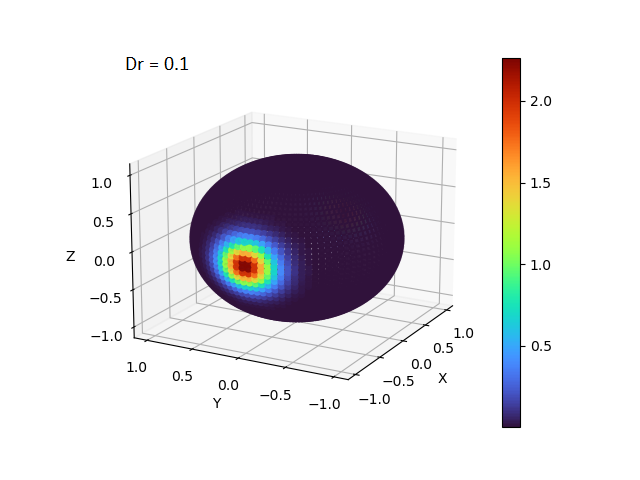
\includegraphics[scale=0.35]{Bilder/exakteLsg_example3.1}
		\end{minipage}
		\hfill 
		\begin{minipage}{0.4\textwidth}
			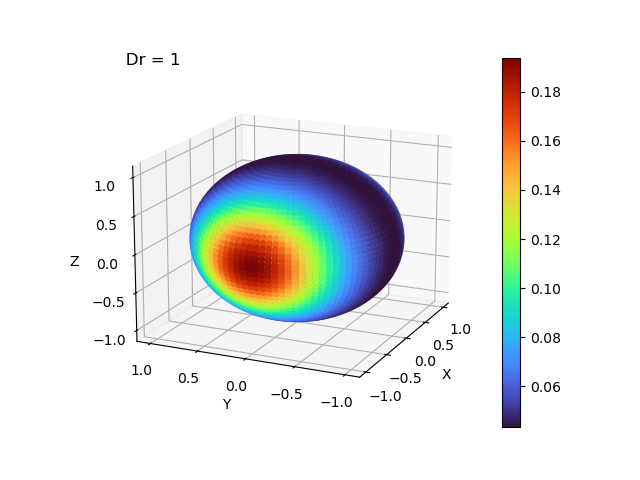
\includegraphics[scale=0.35]{Bilder/exakteLsg_example31_l=1_dr1}
		\end{minipage}
		\caption{Exact steady-state solution for different $D_r$}
	\end{figure}
\end{frame}



\begin{frame}{Elongational flow}
	\begin{figure}
		\begin{minipage}{0.48\textwidth}
			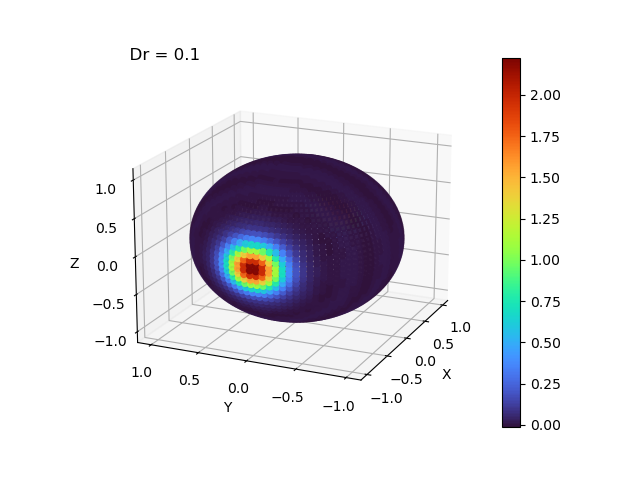
\includegraphics[scale=0.4]{Bilder/example3.1_14nd_linspace(0,10,500)_dr=0.1}
		\end{minipage}
		\hfill 
		\begin{minipage}{0.48\textwidth}
			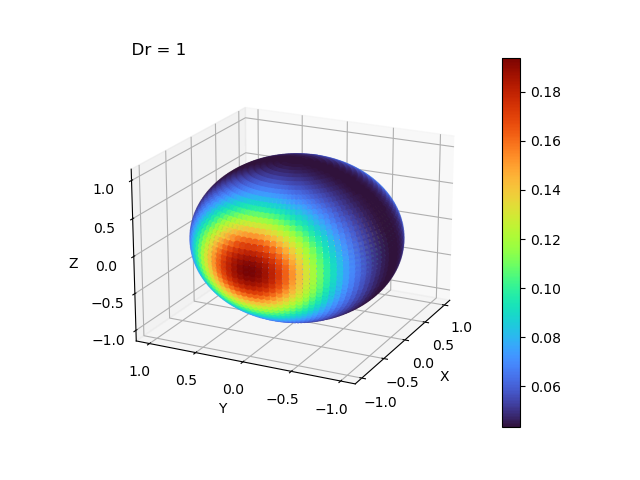
\includegraphics[scale=0.4]{Bilder/example3.1_14nd_linspace(0,10,1000)_dr=1}
		\end{minipage}
		\caption{Numerical solution with basis functions of $14th$ order}
	\end{figure}
\end{frame}

\begin{frame}{Convergence Study}
	For the convergence study, the maximum norm error is used
	\begin{align*}
		E_{max} = max|U_{exact} - U_{approx}|.
	\end{align*}
	
	\begin{figure}
		\begin{minipage}{0.45\textwidth}
			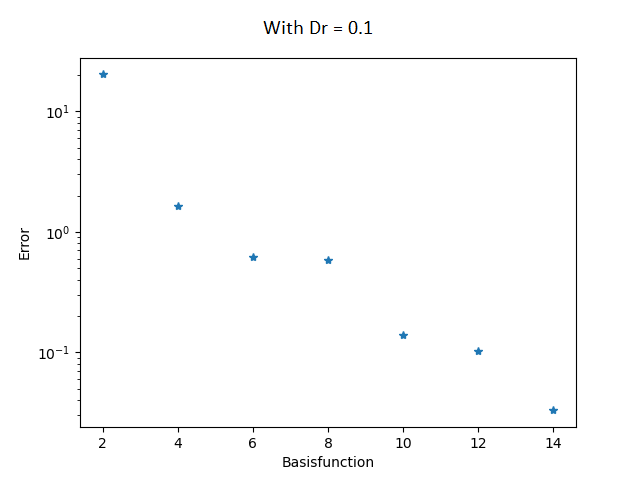
\includegraphics[scale=0.42]{Bilder/Konvergenzstudie_maxnorm_dr=0.1_l=1}
		\end{minipage}
		\hfill 
		\begin{minipage}{0.45\textwidth}
			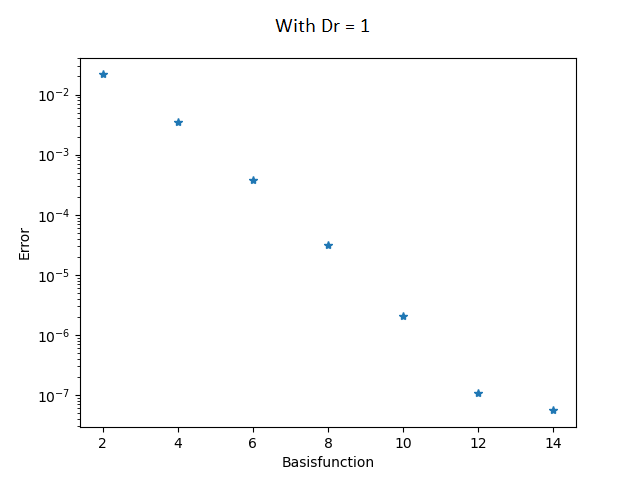
\includegraphics[scale=0.42]{Bilder/Konvergenzstudie_maxnorm_dr=1_l=1}
		\end{minipage}
		\caption{Error with respect to number of basis functions for different $D_r$}
	\end{figure}
\end{frame}

%%%%%%%%%%%%%%%%%%%%%%%%%
% Stability analysis
%%%%%%%%%%%%%%%%%%%%%%%%%

\begin{frame}{Stability analysis}
	\begin{figure}
		\centering
		\subfloat[Coefficients as functions of time]{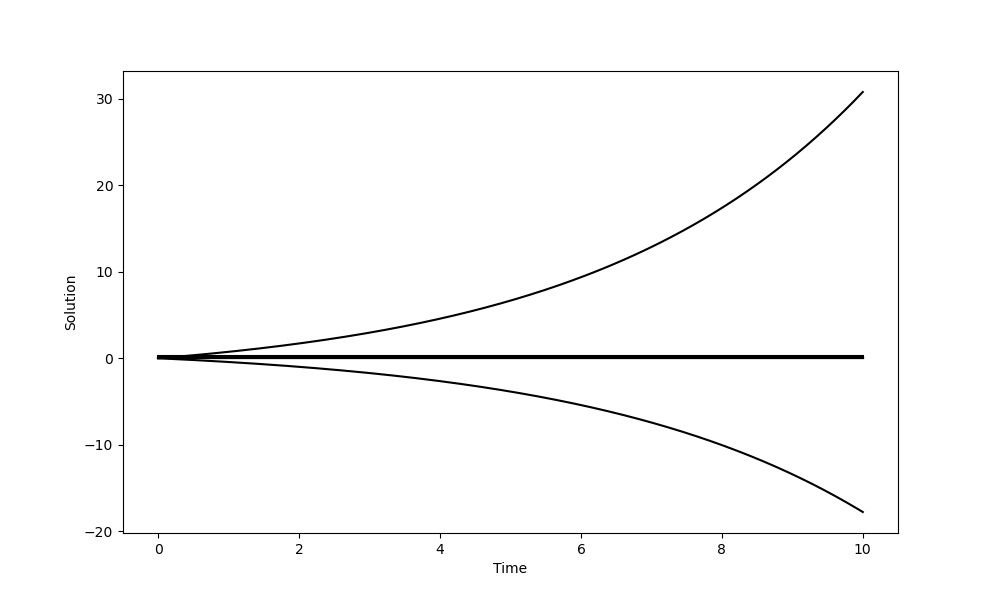
\includegraphics[width=5.5cm,height=4cm]{Bilder/elongational_l=1_ueberZeit_2nd_ohneUeberschrift}}
		\qquad
		\subfloat[Eigenvalues of matrix]{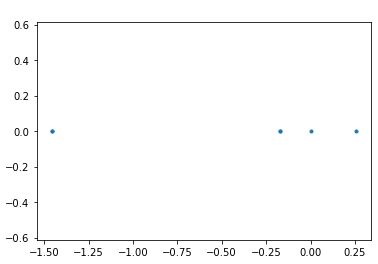
\includegraphics[width=5.5cm,height=3.8cm]{Bilder/eigenvalues_2nd_dr0.1}}
		\caption{For $N=1$ and $D_r$ = 0.1}
	\end{figure}
\end{frame}

\begin{frame}{Stability analysis: Eigenvalues for small $D_r$}
	\begin{figure}
		\begin{subfigure}{0.48\textwidth}
			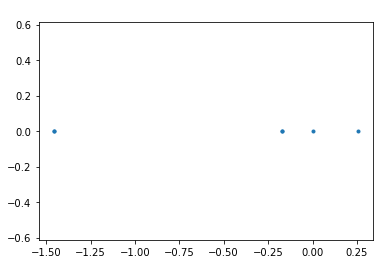
\includegraphics[width=\linewidth]{Bilder/Stability_analysis_2nd_dr0.1}
		\end{subfigure}
		\hfill
		\begin{subfigure}{0.48\textwidth}
			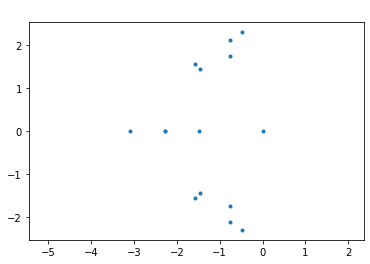
\includegraphics[width=\linewidth]{Bilder/Stability_analysis_4th_dr0.1}
		\end{subfigure}
		\caption{Eigenvalues of matrix $A$ for $D_r = 0.1$}
	\end{figure}

	\begin{block}{Finding}
		Eigenvalues for matrix of $2nd$ order ODE systems $>0$ $\Rightarrow$ ODE unstable
	\end{block}
\end{frame}

\begin{frame}{Stability analysis: Eigenvalues for small $D_r$}
	\begin{figure}
		\begin{subfigure}{0.48\textwidth}
			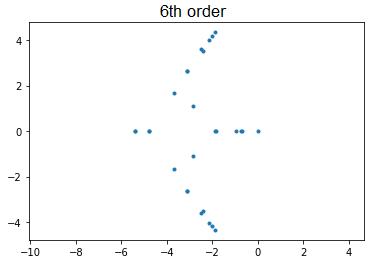
\includegraphics[width=\linewidth]{Bilder/Stability_analysis_6th_dr0.1}
		\end{subfigure}
		\hfill
		\begin{subfigure}{0.48\textwidth}
			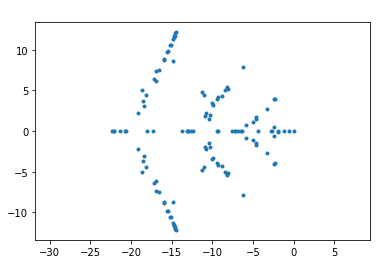
\includegraphics[width=\linewidth]{Bilder/Stability_analysis_14th_dr0.1}
		\end{subfigure}
		\caption{Eigenvalues of matrix $A$ for $D_r = 0.1$}
	\end{figure}
	\begin{block}{Finding}
		An increase of the number of basis functions improves the stability of the spectral method
	\end{block}
\end{frame}

\begin{frame}{Stability analysis: Eigenvalues for large $D_r$}
	\begin{figure}
		\begin{subfigure}{0.48\textwidth}
			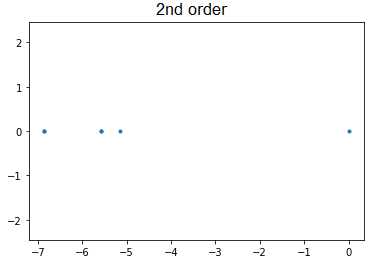
\includegraphics[width=\linewidth]{Bilder/Stability_analysis_2nd_dr1}
		\end{subfigure}
		\hfill
		\begin{subfigure}{0.48\textwidth}
			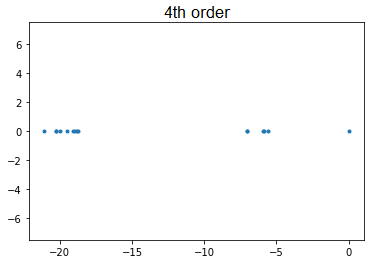
\includegraphics[width=\linewidth]{Bilder/Stability_analysis_4th_dr1}
		\end{subfigure}
		\caption{Eigenvalues of matrix $A$ for $D_r = 1$}
	\end{figure}
\end{frame}

\begin{frame}{Absolute stability: for large $D_r$}
	\begin{figure}
		\begin{subfigure}{0.48\textwidth}
			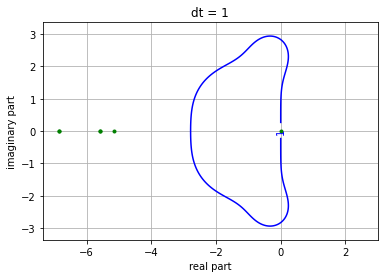
\includegraphics[width=\linewidth]{Bilder/RK4_region_2nd_dr=1_dt=1}
		\end{subfigure}
		\hfill
		\begin{subfigure}{0.48\textwidth}
			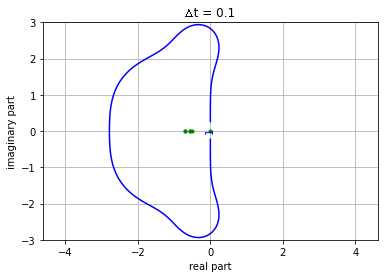
\includegraphics[width=\linewidth]{Bilder/RK4_region_2nd_dr=1_dt=0.1}
		\end{subfigure}
		\caption{Stability region of $RK4$ with eigenvalues for $N=1$, $D_r=1$ and different time steps}
	\end{figure}
\end{frame}

\begin{frame}{Absolute stability: for large $D_r$}
	\begin{figure}
		\begin{subfigure}{0.48\textwidth}
			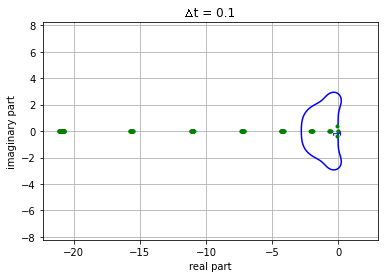
\includegraphics[width=\linewidth]{Bilder/RK4_region_14th_dr=1_dt=0.1}
		\end{subfigure}
		\hfill
		\begin{subfigure}{0.48\textwidth}
			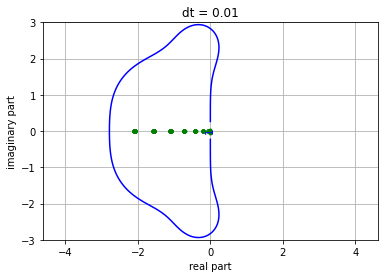
\includegraphics[width=\linewidth]{Bilder/RK4_region_14th_dr=1_dt=0.01}
		\end{subfigure}
		\caption{Stability region of $RK4$ with eigenvalues for $N=7$, $D_r=1$ and different time steps}
	\end{figure}

	\begin{block}{Finding}
	For absolute stability for large $D_r$  $\rightarrow$ smaller time steps are needed
	\end{block}
\end{frame}


%%%%%%%%%%%%%%%%%%%%%%%%%%%%%%%%%%%%%%
% Coefficients as functions of time
%%%%%%%%%%%%%%%%%%%%%%%%%%%%%%%%%%%%%%

\begin{frame}
		\begin{figure}
			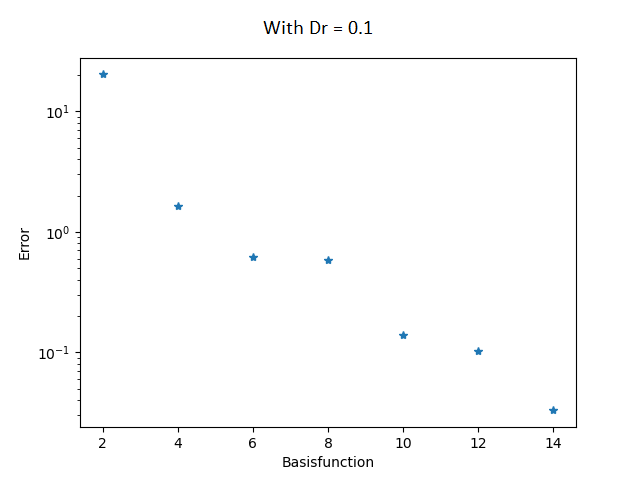
\includegraphics[scale=0.5]{Bilder/Konvergenzstudie_maxnorm_dr=0.1_l=1}
			\caption{Error with respect to number of basis functions for $D_r = 0.1$}
		\end{figure}
	
		\begin{itemize}
			\item for small Dr $\rightarrow$ large inaccuracy
			\item the smallest error is between $10^{-1}$ and $10^{-2}$
		\end{itemize}
\end{frame}

\begin{comment}
\begin{frame}{Coefficients as functions of time}
	\begin{figure}
		\begin{subfigure}{0.48\textwidth}
			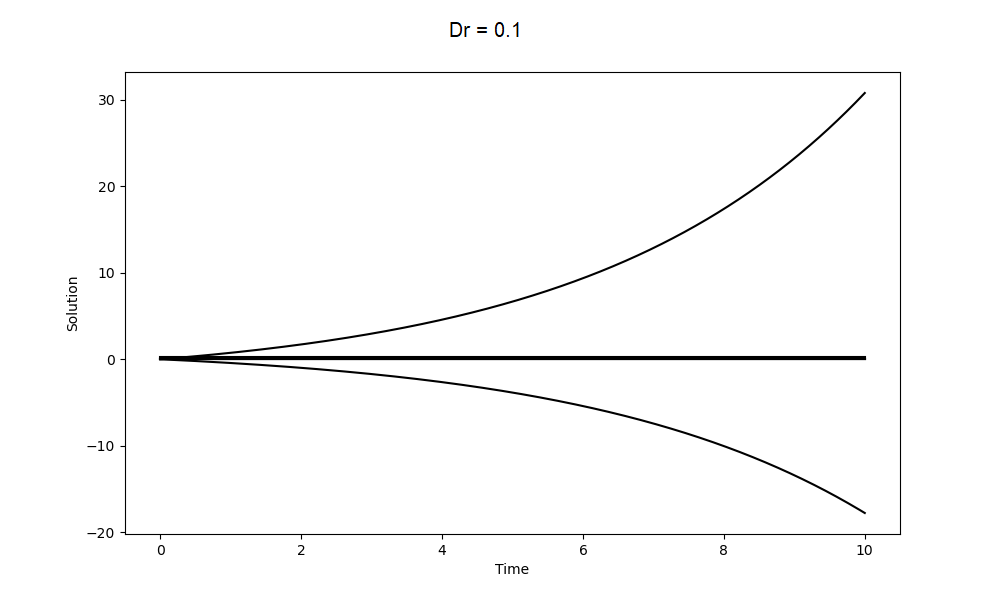
\includegraphics[width=\linewidth]{Bilder/elongational_l=1_lsg_ueber_Zeit_2nd}
		\end{subfigure}
		\hfill
		\begin{subfigure}{0.48\textwidth}
			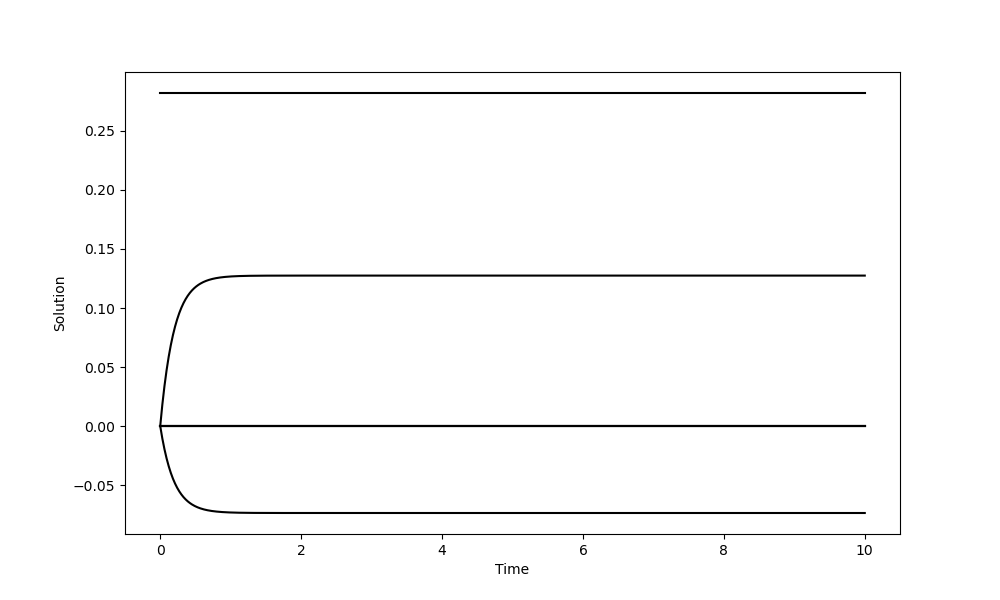
\includegraphics[width=\linewidth]{Bilder/elongational_l=1_lsg_ueber_Zeit_2nd_dr=1}
		\end{subfigure}
		\caption{Coefficients as functions of time for $N=1$}
	\end{figure}
\end{frame}
\end{comment}


\begin{frame}{Coefficients as functions of time}
	\begin{figure}
		\begin{subfigure}{0.48\textwidth}
			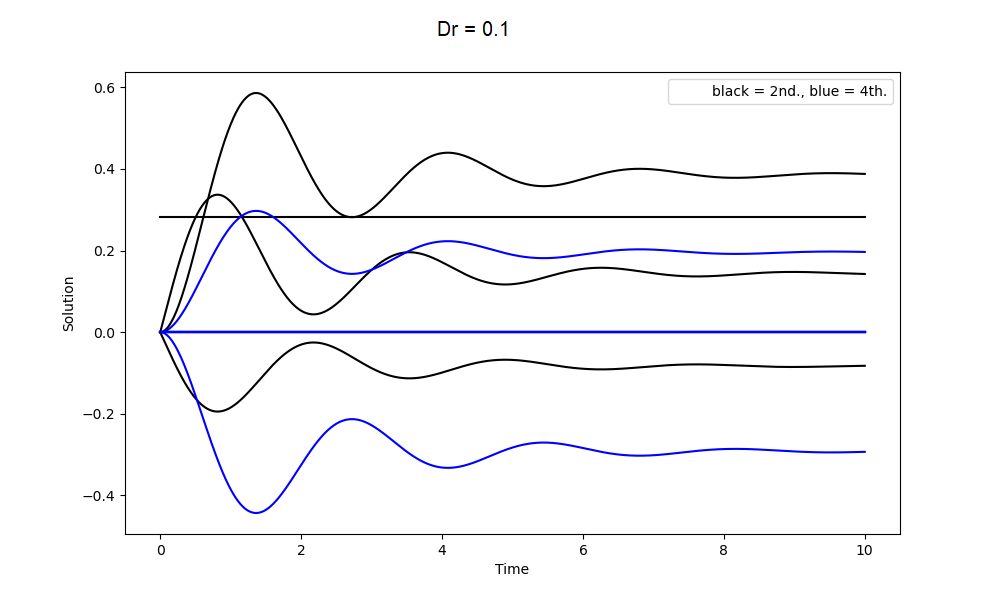
\includegraphics[width=\linewidth]{Bilder/elongational_l=1_lsg_ueber_Zeit_4th}
		\end{subfigure}
		\hfill
		\begin{subfigure}{0.48\textwidth}
			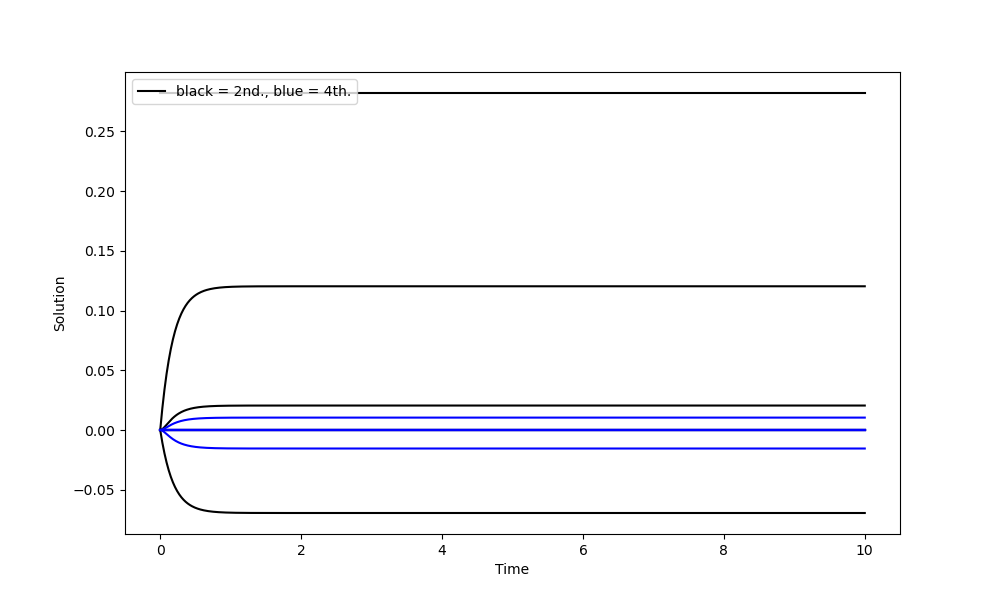
\includegraphics[width=\linewidth]{Bilder/elongational_l=1_lsg_ueber_Zeit_4th_dr=1}
		\end{subfigure}
		\caption{Coefficients as functions of time for $N=2$}
	\end{figure}
\end{frame}

\begin{comment}
\begin{frame}{Coefficients as functions of time}
	\begin{figure}
		\begin{subfigure}{0.48\textwidth}
			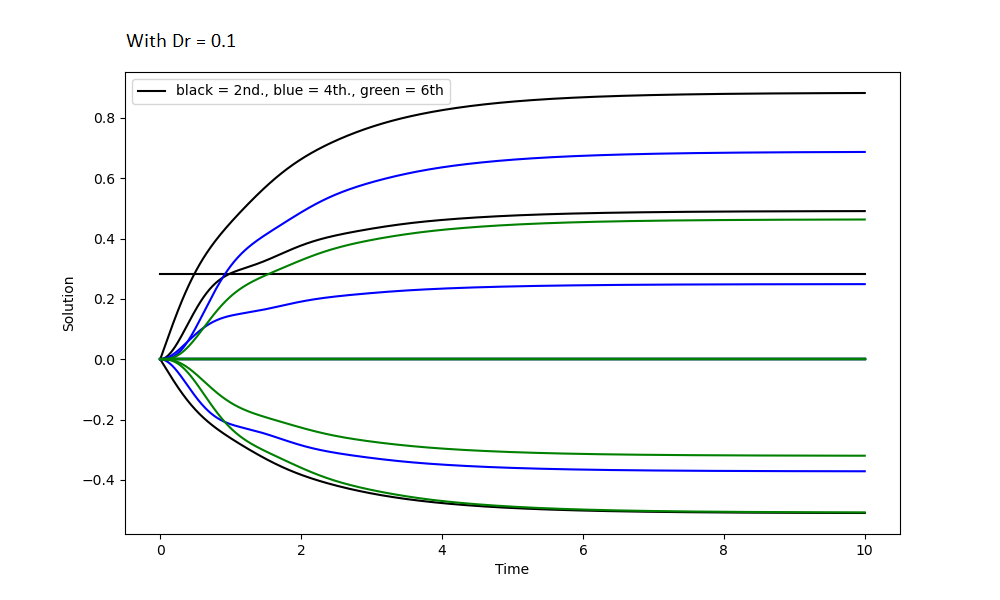
\includegraphics[width=\linewidth]{Bilder/elongational_l=1_lsg_ueber_Zeit_6th}
		\end{subfigure}
		\hfill
		\begin{subfigure}{0.48\textwidth}
			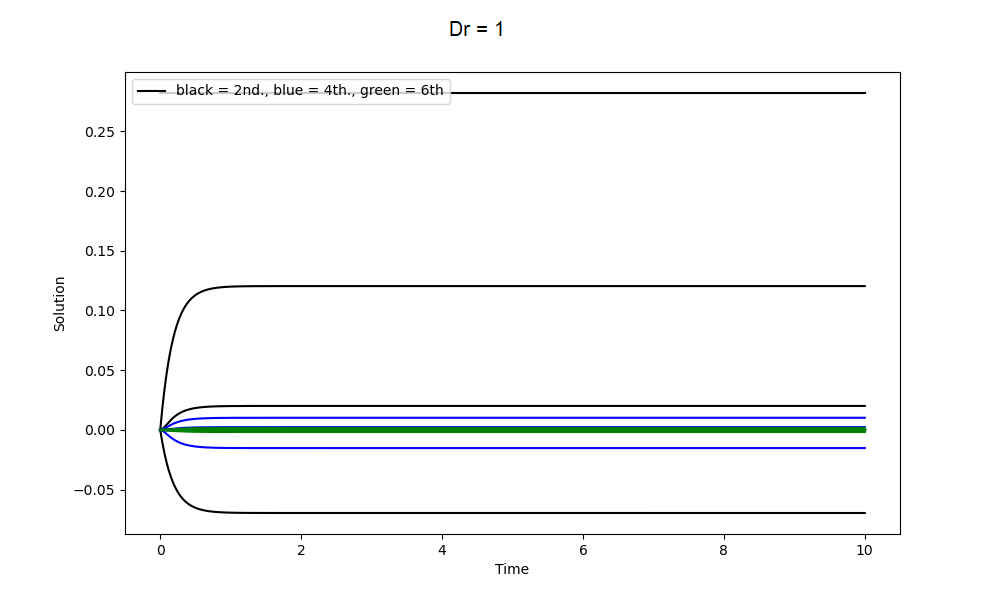
\includegraphics[width=\linewidth]{Bilder/elongational_l=1_lsg_ueber_Zeit_6th_dr=1}
		\end{subfigure}
		\caption{Coefficients as functions of time for $6th$ order}
	\end{figure}
\end{frame}
\end{comment}

\begin{frame}{Coefficients as functions of time}
	\begin{figure}
		\begin{subfigure}{0.48\textwidth}
			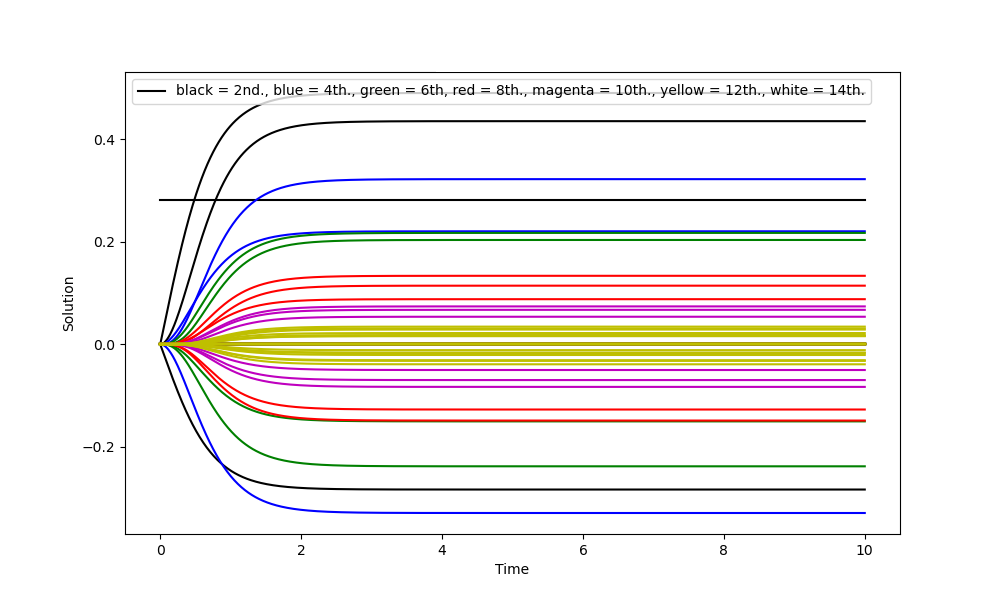
\includegraphics[width=\linewidth]{Bilder/elongational_l=1_lsg_ueber_Zeit_14th}
		\end{subfigure}
		\hfill
		\begin{subfigure}{0.48\textwidth}
			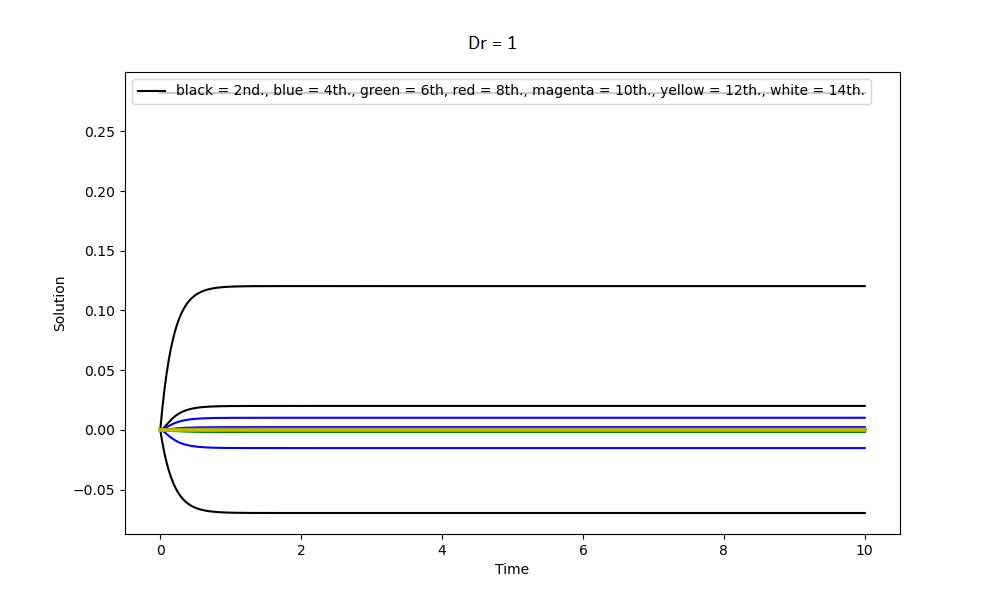
\includegraphics[width=\linewidth]{Bilder/elongational_l=1_lsg_ueber_Zeit_14th_dr=1}
		\end{subfigure}
		\caption{Coefficients as functions of time for $N=7$}
	\end{figure}
\end{frame}





%%%%%%%%%%%%%%%%%%%%%%%%%%%%%%%%%%%%%
%%%%%%%%%%%%%%%%%%%%%%%%%%%%%%%%%%%%%
% Shear flow on S^1
%%%%%%%%%%%%%%%%%%%%%%%%%%%%%%%%%%%%%
%%%%%%%%%%%%%%%%%%%%%%%%%%%%%%%%%%%%%

\begin{comment}
\subsection{Shear flow on $S^1$ and $S^2$}

\begin{frame}
	\centering
	Shear flow on $S^1$
\end{frame}

\begin{frame}{Shear flow on $S^1$}
	\scriptsize
	The externally imposed velocity gradient has the form
	\begin{figure}
	\centering
	\begin{equation}
	\nabla_{\mathbf{x}} \mathbf{u}=\begin{pmatrix}
		0 & 1 & 0 \\
		0 & 0 & 0 \\
		0 & 0 & 0
	\end{pmatrix}
	\end{equation}
	\end{figure}

TODO
\end{frame}

\subsubsection{Stability analysis}
\begin{frame}{Shear flow  on $S^1$: Stability analysis}
	\begin{figure}
		\centering
		\begin{minipage}{0.4\linewidth}
			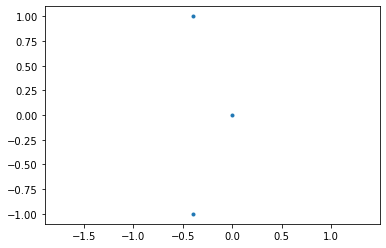
\includegraphics[scale=.42]{Bilder/Stability_analysis_shearflow_N=1_dr0.1}
		\end{minipage}
		\hspace{1cm}
		\begin{minipage}{0.4\linewidth}
			\centering
			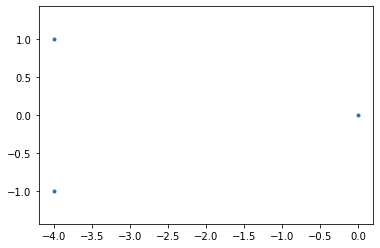
\includegraphics[scale=0.42]{Bilder/Stability_analysis_shearflow_N=1_dr1}
		\end{minipage}
		\caption{Eigenvalue of matrix $A$ with $N=1$}
	\end{figure}
	
	\begin{block}{Proposition 2}
		Sprectal method for $N=1$ is stable with for both small and large $D_r$.
	\end{block}
\end{frame}


\begin{frame}{Shear flow  on $S^1$: Stability analysis}
	\begin{figure}
		\centering
		\begin{minipage}{0.4\linewidth}
			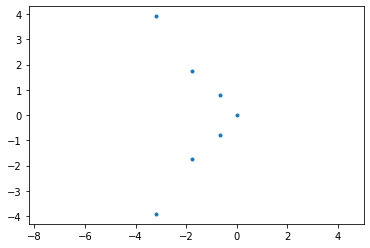
\includegraphics[scale=.42]{Bilder/Stability_analysis_shearflow_N=3_dr0.1}
		\end{minipage}
		\hspace{1cm}
		\begin{minipage}{0.4\linewidth}
			\centering
			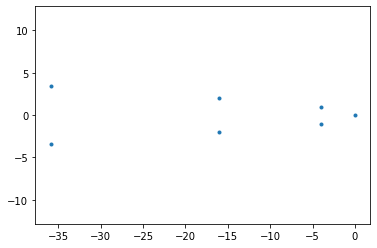
\includegraphics[scale=0.42]{Bilder/Stability_analysis_shearflow_N=3_dr1}
		\end{minipage}
		\caption{Eigenvalue of matrix $A$ $N=3$}
	\end{figure}
	
	\begin{block}{Proposition 3}
		Sprectal method for $N=3$ is stable with for both small and large $D_r$.
	\end{block}
\end{frame}
	Inhalt...
\end{comment}

%%%%%%%%%%%%%%%%%%%%%%%%%%%%%%%%%%%%%
%%%%%%%%%%%%%%%%%%%%%%%%%%%%%%%%%%%%%
% Shear flow on S^2 
%%%%%%%%%%%%%%%%%%%%%%%%%%%%%%%%%%%%%
%%%%%%%%%%%%%%%%%%%%%%%%%%%%%%%%%%%%%


\begin{frame}
	\centering
	Shear flow on $S^2$
\end{frame}

\begin{frame}{Shear flow on $S^2$}
	\scriptsize
	Consider the externally imposed shear flow 
	\begin{figure}
		\centering
		\begin{equation}
			\mathbf{u}=\begin{pmatrix}
				u(y) \\
				0 \\
				0
			\end{pmatrix}, \quad \nabla_{\mathbf{x}} \mathbf{u}=\begin{pmatrix}
				0 & 1 & 0 \\
				0 & 0 & 0 \\
				0 & 0 & 0
			\end{pmatrix}
		\end{equation}
	\end{figure}

\begin{figure}
	\small
	\begin{minipage}{0.43\textwidth}
		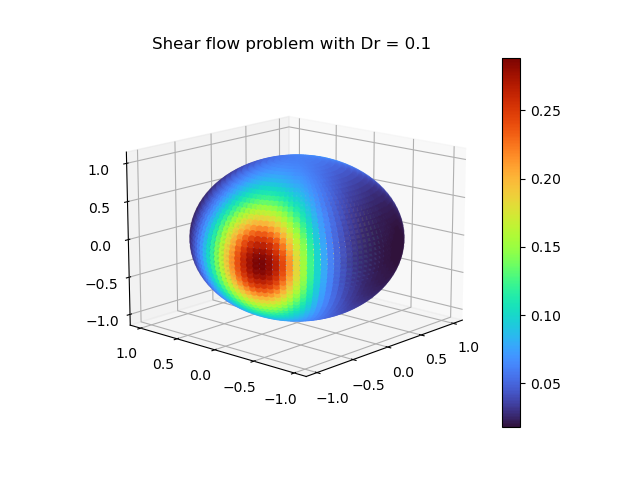
\includegraphics[scale=0.35]{Bilder/shearflow_12th_dr0.1}
	\end{minipage}
	\hfill 
	\begin{minipage}{0.43\textwidth}
		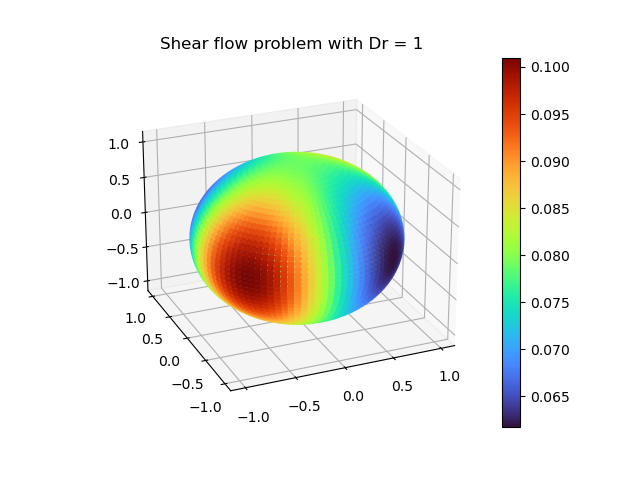
\includegraphics[scale=0.35]{Bilder/shearflow_12th_linspace(0,10,500)_dr=1}
	\end{minipage}
	\caption{Steady state solution of the Smoluchowski equation approximated at $T = 10$ using different values of $D_r$.}
\end{figure}
\end{frame}

\begin{frame}{Shear flow: Stability analysis}
	\begin{figure}
		\centering
		\begin{minipage}{0.4\linewidth}
			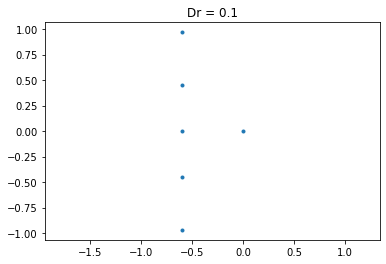
\includegraphics[scale=.42]{Bilder/Stability_analysis_shearflow_2nd_dr0.1}
		\end{minipage}
		\hspace{1cm}
		\begin{minipage}{0.4\linewidth}
			\centering
			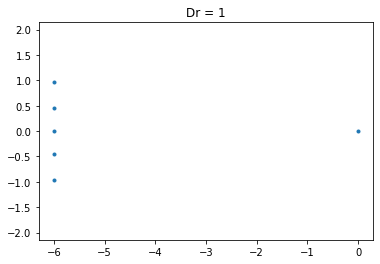
\includegraphics[scale=0.42]{Bilder/Stability_analysis_shearflow_2nd_dr1}
		\end{minipage}
		\caption{Eigenvalues of matrix $A$ for $N=1$}
	\end{figure}
	
	\begin{block}{Finding}
		Spectral method for $N=1$ is stable for any $D_r$.
	\end{block}
\end{frame}

\begin{frame}{Shear flow: Stability analysis}
	\begin{figure}
		\centering
		\begin{minipage}{0.4\linewidth}
			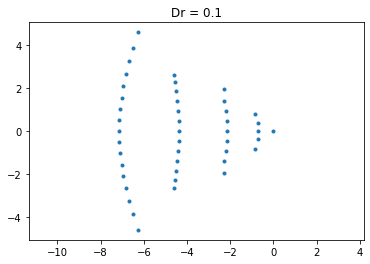
\includegraphics[scale=.42]{Bilder/Stability_analysis_shearflow_8th_dr0.1}
		\end{minipage}
		\hspace{1cm}
		\begin{minipage}{0.4\linewidth}
			\centering
			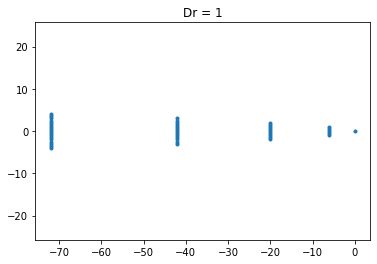
\includegraphics[scale=0.42]{Bilder/Stability_analysis_shearflow_8th_dr1}
		\end{minipage}
		\caption{Eigenvalues of matrix $A$ for $N=4$}
	\end{figure}
	
	\begin{block}{Finding}
		Spectral method for $N=4$ is stable for any $D_r$.
	\end{block}
\end{frame}



%%%%%%%%%%%%%%%%%%%%%%%%%%%%%%%%%%



\begin{comment}
\begin{frame}{Elongational flow: Stability analysis}
	\begin{columns}
		\begin{column}{0.5\textwidth}
			\begin{figure}
				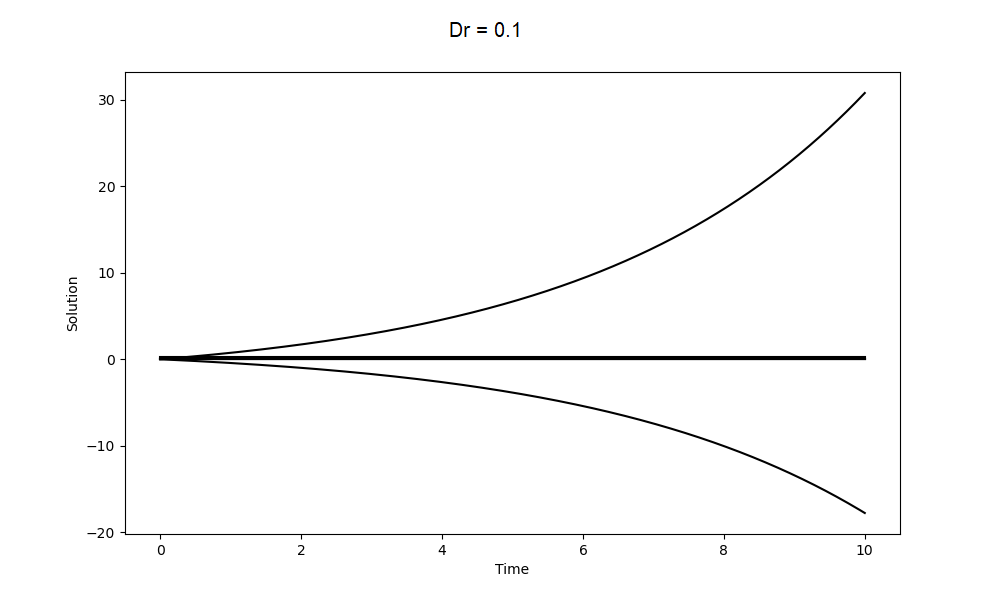
\includegraphics[width=0.97\linewidth]{Bilder/elongational_l=1_lsg_ueber_Zeit_2nd}
				\caption{Coefficients as function of time}
			\end{figure}
		\end{column}
		\begin{column}{0.5\textwidth}
			\begin{figure}
				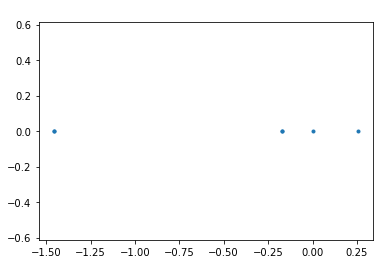
\includegraphics[width=0.8\linewidth]{Bilder/Stability_analysis_2nd_dr0.1}
				\caption{Eigenvalue of matrix $A$}
			\end{figure}
		\end{column}
	\end{columns}
	\centering
	With $2nd.$ order and $D_r = 0.1$.
\end{frame}

\begin{frame}{Elongational flow: Stability analysis}
	\begin{columns}
		\begin{column}{0.5\textwidth}
			\begin{figure}
				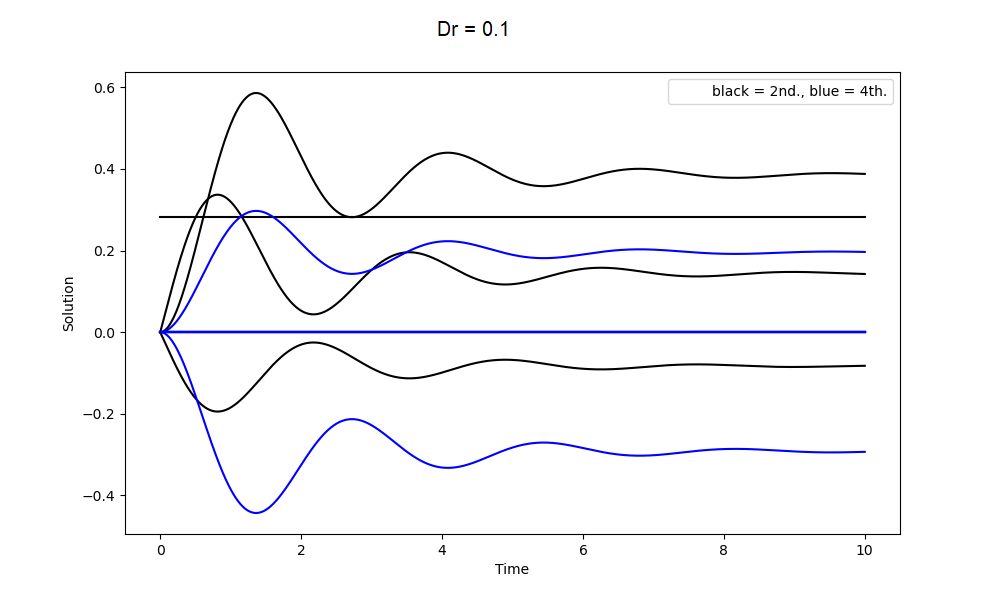
\includegraphics[width=0.97\linewidth]{Bilder/elongational_l=1_lsg_ueber_Zeit_4th}
				\caption{Coefficients as function of time}
			\end{figure}
		\end{column}
		\begin{column}{0.5\textwidth}
			\begin{figure}
				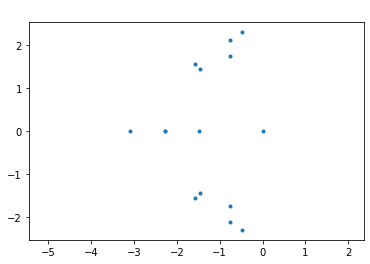
\includegraphics[width=0.8\linewidth]{Bilder/Stability_analysis_4th_dr0.1}
				\caption{Eigenvalue of matrix $A$}
			\end{figure}
		\end{column}
	\end{columns}
	\centering
	With $4th.$ order and $D_r = 0.1$.
\end{frame}


\begin{frame}{Elongational flow: Stability analysis}
	\begin{columns}
		\begin{column}{0.5\textwidth}
			\begin{figure}
				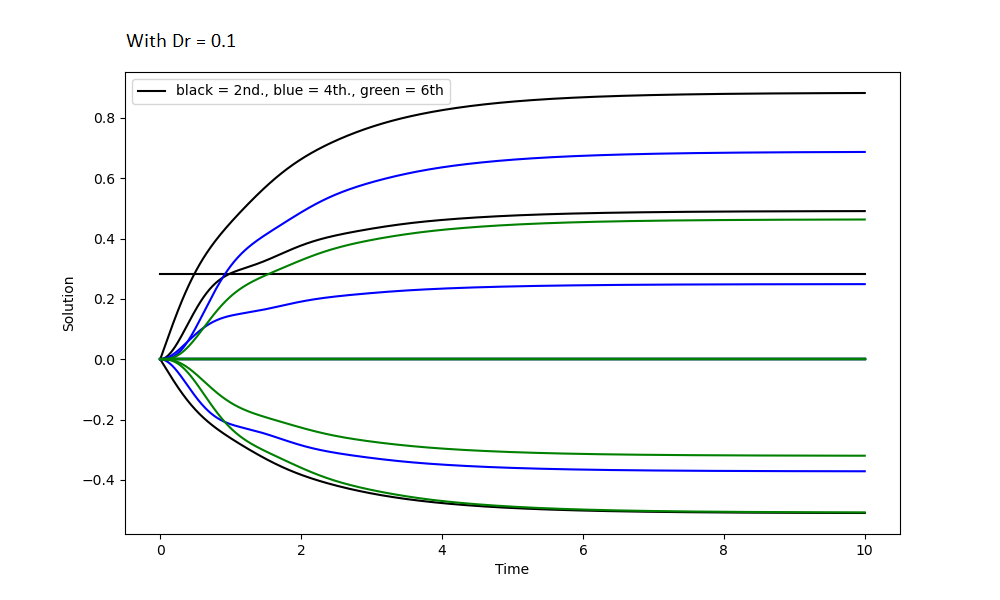
\includegraphics[width=0.97\linewidth]{Bilder/elongational_l=1_lsg_ueber_Zeit_6th}
				\caption{Coefficients as function of time}
			\end{figure}
		\end{column}
		\begin{column}{0.5\textwidth}
			\begin{figure}
				\includegraphics[width=0.82\linewidth]{Bilder/Stability_analysis_6th_dr0.1}
				\caption{Eigenvalue of matrix $A$}
			\end{figure}
		\end{column}
	\end{columns}
	\centering
	With $6th.$ order and $D_r = 0.1$.
\end{frame}

\begin{frame}{Elongational flow: Stability analysis}
	\begin{columns}
		\begin{column}{0.5\textwidth}
			\begin{figure}
				\includegraphics[width=0.97\linewidth]{Bilder/elongational_l=1_lsg_ueber_Zeit_14th}
				\caption{Coefficients as function of time}
			\end{figure}
		\end{column}
		\begin{column}{0.5\textwidth}
			\begin{figure}
				\includegraphics[width=0.83\linewidth]{Bilder/Stability_analysis_14th_dr0.1}
				\caption{Eigenvalue of matrix $A$}
			\end{figure}
		\end{column}
	\end{columns}
	\centering
	With $14th.$ order and $D_r = 0.1$.
\end{frame}
\end{comment}


\begin{comment}
\begin{frame}{Elongational flow: Stability analysis}
	\begin{figure}
		\centering
		\begin{minipage}{0.4\linewidth}
			\includegraphics[scale=.42]{Bilder/Stability_analysis_2nd_dr1}
		\end{minipage}
		\hspace{1cm}
		\begin{minipage}{0.4\linewidth}
			\centering
			\includegraphics[scale=0.42]{Bilder/Stability_analysis_2nd_dr0.14}
		\end{minipage}
		\caption{Eigenvalue of matrix $A$ with basis functions of $2nd.$ order}
	\end{figure}
	
	\begin{block}{Finding 1}
		The maximum value of eigenvalue of matrix $A$ with basis functions of $2nd.$ order is $0.01714 > 0$. It follows:
		Sprectal method for $2nd.$ order is unstable with $D_r < 0.15$.
	\end{block}
\end{frame}
\end{comment}


\begin{frame}{Conclusion}
		\begin{itemize}
			\item Derivation of the spectral method is the first step to derive the moment system
			\item In order for the method to be stable,
				\begin{itemize}
					\item for small $D_r$ more approach functions 
					\item for large $D_r$ smaller time steps 
				\end{itemize} 
			are needed
		\end{itemize}
\end{frame}


%\begin{frame}
%	\begin{figure}[h]
%		\centering
%		\includegraphics[scale=.35]{Bilder/Solution_over_time_14th}
%		\caption{Numerical solution of ODE systems over time with $D_r$ = 1}
%		\label{fig: Solution of ODE systems over time with $D_r$ = 1}
%	\end{figure}
%\end{frame}


%\section{Example}
\begin{frame}
	\scriptsize	With velocity gradient
	\begin{align*}
		\scriptsize \nabla_{\vec{x}} \vec{u}_{ext} = \left( \begin{array}{rrr}
			0 & 1 & 0 \\ 
			0 & 0 & 0 \\
			0 & 0 & 0 \\ 
		\end{array}\right)
	\end{align*}
	\begin{figure}
	\subfloat[]{\includegraphics[scale=0.35]{Bilder/shearflow_4th_linspace(0,10,500)}}
	\qquad
	\subfloat[]{\includegraphics[scale=0.35]{Bilder/shearflow_4th_linspace(0,10,500)_dr=1}}
	\scriptsize \caption{Numerical solution of the Smoluchowski equation with Spectral method with harmonic polynomial basis functions $a)$ $b)$ $4th$.}
	\end{figure}
\end{frame}


\begin{frame}
	\begin{minipage}{0.4\textwidth}
		\includegraphics[scale=0.4]{Bilder/shearflow_10th_linspace(0,10,500)}
	\end{minipage}
	\hfill 
	\begin{minipage}{0.4\textwidth}
		\includegraphics[scale=0.4]{Bilder/shearflow_10th_linspace(0,10,500)_dr=1}
	\end{minipage}
\end{frame}







\begin{frame}
	\centering
	Thank you for listening!
\end{frame}

\AtBeginSection[]
%{
% \begin{frame}<beamer>
% \frametitle{Table of Contents}
% \tableofcontents[currentsection]
% \end{frame}
%}



%Ende
%\begin{frame}{Ende}
%	\centering
%	Thank you for listening!
%\end{frame}


\begin{frame}[allowframebreaks]
  \frametitle{Literatur}
  \nocite{*} %es werden auch Quellen aufgefuehrt, die nicht in den Folien zitiert sind.
  \bibliography{Bibliothek}
  \bibliographystyle{abbrv}
\end{frame}

\end{document}